\documentclass{report}

\usepackage[slovene, provide=*]{babel}
\usepackage{minted}
\usepackage{graphicx}
\graphicspath{ {./images} }
\usepackage{csquotes}
\usepackage[backend=bibtex]{biblatex}
\addbibresource{literatura.bib}
\nocite{*}
\usepackage{authblk}

\title{Izdelava operacijskega sistema}
\author{Luka Golob Cerar, 4.b}
\affil{Mentor: Vincenc Kušar}
% Dodej kušarja


\begin{document}
\begin{titlepage}
   \begin{center}
       \hspace*{1.5cm}
\includegraphics[width=0.6\textwidth]{gssrm}

       \textbf{Izdelava operacijskega sistema}

       \vspace{1.5em}

       \textbf{Luka Golob Cerar}

       \vfill
            
       Oddelek: 4.b\\
       Mentor: Vincenc Kušar\\
       Gimnazija in srednja šola Rudolfa Maistra\\
       Novi trg 41a, 1241 Kamnik
   \end{center}
\end{titlepage}

\tableofcontents

\chapter{Uvod}

\section{Dispozicija}
Operacijski sistem je program, ki ga vsi uporabljamo (npr. Windows, GNU/Linux...), a o njem ne razmišljamo kaj preveč zaradi njegove kompleksnosti. A kaj sploh je operacijski sistem in kako deluje?

Operacijski sistem (OS) je programska oprema potrebna za delovanje in uporabo
računalnika. Deluje kot vmesnik med računalniško strojno opremo in uporabnikom.
Ima več ključnih nalog, med katerimi so upravljanje procesov, upravljanje
pomnilnika, upravljanje datotečnega sistema, upravljanje vhodno-izhodnih naprav
ter zagotavljanje varnosti in zaščite sistema. Ti elementi skupaj tvorijo osnovo
za delovanje vsakega računalnika in omogočajo uporabnikom učinkovito izvajanje
različnih opravil. Srce operacijskega sistema tvori njegovo ``jedro''. Jedro upravlja delovanje računalnika in strojne opreme. Jedro se najprej naloži v pomnilnik, ko se naloži operacijski sistem, in ostane v pomnilniku, dokler se operacijski sistem ponovno ne izklopi. Odgovorno je za različna opravila, kot so upravljanje diskov, upravljanje opravil in upravljanje pomnilnika.

V tej nalogi bom dokumentiral izdelavo zelo preprostega operacijskega sistema. Začel bom s pripravo delovnega okolja, nato bom izdelal preprost prototip, ki ga računalnik lahko zažene in ne naredi nič več (gre v neskončno zanko). Za temu bom program prilagodil, da na ekranu računalnika izpiše pozdrav. V zadnjem (in najbolj obsežnem) delu bom iz 16-bitnega načina preklopil na 32-bitni, napisal vmesnik za branje z diska in za konec z navkrižno kompilacijo napisal preprosto jedro operacijskega sistema v programskem jeziku C.

\section{Priprava okolja}
Za začetek si moramo pripraviti svoje programsko okolje. Jaz uporabljam Arch Linux in zato bodo nekateri ukazi specifični za mojo konfiguracijo.

Komuniciranje z strojno opremo je zelo nizko stopenjsko opravilo, ki je mogoče
le ob uporabi zbirnega jezika. Zbirni jezik je nizkonivojski programski jezik,
ki predstavlja najboljši približek dobesednemu prevodu navodil, ki jih
računalnik izvaja, v človeku razumljivi obliki. Za ta projekt bom uporabljal
NASM. NASM (Netwide Assembler) je ``asembler'' za 80x86 in x86-64 arhitekture, zasnovan za prenosljivost in modularnost. Podpira vrsto formatov objektnih datotek, vključno z Linuxom in *BSD a.out, ELF, Mach-O, 16-bitnim in 32-bitnim formatom .obj (OMF), COFF (vključno z različicama Win32 in Win64), izpisuje lahko tudi navadne binarne datoteke, kar je za ta projekt najbolj pomembno, saj bomo ta format tudi uporabljali. Njegova sintaksa je zasnovana tako, da je preprosta in lahko razumljiva.

Naložimo ga z naslednjim ukazom:
    \begin{minted}{bash}
        sudo pacman -S nasm
    \end{minted}

Kasneje bomo uporabljali še en, sicer eno stopnjo višji, programski jezik – C.
Naložimo prevajalnik še za ta jezik:
    \begin{minted}{bash}
        sudo pacman -S gcc
    \end{minted}

Izdelava operacijskega sistema bi bila skoraj nemogoča, če bi bilo potrebno računalnik ob vsaki spremembi znova zagnati iz Linux sistema v operacijski sistem, ki ga pišemo. Zaradi tega bomo računalnik simulirali s programom QEMU. QEMU emulira procesor računalnika in zagotavlja nabor različnih modelov strojne opreme in naprav za računalnik, kar omogoča zagon različnih gostujočih operacijskih sistemov, vključno z našim.
    \begin{minted}{bash}
        sudo pacman -S qemu-full
    \end{minted}
Potrebovali bomo še en program za pisanje kode. Jaz sem se odločil za Neovim, a izbira ni pomembna.

\chapter{BIOS in zagonska rutina}

\section{BIOS in zagonski bloki}
Ob zagonu računalnika v spominu ni naloženega nobenega programa, ki bi ga lahko procesor zagnal, zato si pomaga z osnovno vhodno/izhodno programsko opremo (BIOS), ki je naložena na matični plošči. BIOS je zbirka programskih rutin, ki se na začetku naložijo s čipa v pomnilnik in se inicializirajo ob vklopu računalnika. BIOS omogoča samodejno zaznavanje in osnovni nadzor naprav računalnika, kot so zaslon, tipkovnica in trdi diski. Ko BIOS opravi nekaj testov strojne opreme na nizki ravni, npr. ali nameščeni pomnilnik deluje pravilno, mora zagnati operacijski sistem, ki je shranjen na eni od naprav. Pri tem moramo paziti, da BIOS ne more preprosto naložiti datoteke, ki predstavlja operacijski sistem z diska, saj BIOS nima ideje o datoteki, ker brez operacijskega sistema tudi datotečne strukture ni. BIOS mora prebrati določene sektorje podatkov (običajno velikosti 512 bajtov) iz določenih fizičnih lokacij na disku. Če je na koncu tega sektorja število 0xaa55 (heksadecimalno), to prepozna za zagonski blok, ki ga nato premakne v pomnilnik in naroči procesorju, naj ga začne izvajati od začetka. Tu prevzamemo nadzor nad računalnikom.

\section{Zagonska rutina}
Ta proces lahko tudi preizkusimo. Na gostiteljskem sistemu (Arch Linux) sem ustvaril datoteko po imenu »hello.asm«. To datoteko sem odprl v programu za oblikovanje besedila in vanj vpisal:
\begin{minted}{nasm}
    jmp $ ; neskončna zanka

    times 510-($-$$) db 0 ; Poskrbi za pravilno obliko datoteke
    dw 0xaa55             ; Število po katerem BIOS zazna datoteko
                          ; kot zagonski sektor.
\end{minted}

Poglejmo vsako vrstico posebej. V prvi liniji imamo programski ukaz ``jmp''. Ta
sporoči procesorju naj skoči nekam drugam v programu in nadaljuje izvajanje
ukazov od tam naprej. Kot argument ima podan znak \$. Ta znak predstavlja naslov trenutne vrstice v spominu. Procesor bo prebral ukaz in argument, nato skočil nazaj na isto mesto in to ponavljal v nedogled.

Na tretji vrstici imamo v resnici dva ukaza, prvi je ``times'', drugi pa ``db''.
Times ni zares ukaz za procesor, ampak za NASM. Argument tega ukaza, v našem
primeru ``510-(\$-\$\$)'', NASM-u pove kolikokrat mora ponoviti naslednji ukaz
(``db 0''). Se pravi, da je tretja vrstica ista kakor da bi ukaz ``db 0'' ponovil
tolikokrat, kolikor je podano v argumentu. A katero število predstavlja naš
argument? Naš argument je v bistvu enačba treh števil, prvo je 510, temu pa
odštejemo razliko dveh drugih, prvo je število, ki smo ga že spoznali (pozicija
trenutne vrstice v spominu) in ga predstavlja znak \$. Naslednje število
predstavlja znak \$\$ in pomeni začetek trenutnega razdelka; tako lahko z
uporabo (\$-\$\$) ugotovimo, kako daleč v razdelku se nahajamo oz. koliko bajtov je naš program že dolg.

To je pomembno zaradi prej omenjene velikosti sektorja (512 bajtov). (\$-\$\$)
izračuna koliko tega prostora smo že porabili (z ``jmp'' ukazom in argumentom).
To število odštejemo od števila 510 (ne 512, saj zadnja dva bajta definiramo z
zadnjim ukazom) in dobimo število bajtov, ki jih je potrebno napolniti z nečem,
da bo sektor pravilne velikosti. Za to uporabljamo ukaz ``db 0''. DB stoji za
``define byte'' in preprosto v spomin zapiše bajt, ki smo ga podali kot argument, v našem primeru število 0.

Zadnji ukaz, na 4. vrstici je ``dw 0xaa55''. DW deluje zelo podobno kot DB, le
da v spomin ne zapiše bajta, ampak ``besedo'', ki je velika 2 bajta. Število, ki smo ga podali je število, potrebno za prepoznavo s strani BIOS-a (0xaa55).
Z uporabo naslednjega ukaza lahko to kodo spremenimo v obliko, ki jo razume računalnik:
    \begin{minted}{bash}
        nasm hello.asm -f bin -o out.bin
    \end{minted}
Z ``-f bin'' zastavico smo podali format, ki si ga želimo in z ``-o out.bin'' ime datoteke, v katero bo program zapisan. Če generirano datoteko odpremo v programu za branje binarnih datotek (jaz uporabljam ``hexyl''), lahko vidimo naslednje:

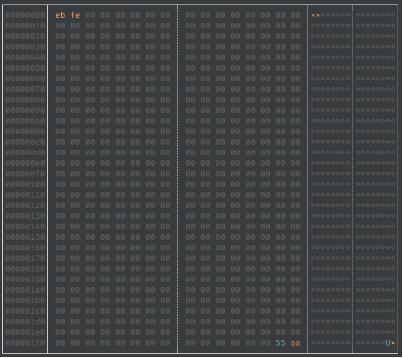
\includegraphics[scale=0.5]{bytes_raw}

Prva dva bajta predstavljata ukaz za skok. Sledi jima 508 ničih bajtov (ker je
512-4 enako 508) in nazadnje bajta 0x55 in 0xaa. Obrnjena sta obratno od našega števila 0xaa55, ker je x86 struktura malo endijska (spodnji del števila je na začetku). Ta program lahko sedaj že zaženemo na računalniku. Namesto da ponovno zaženemo gostiteljski računalnik, uporabimo QEMU z naslednjim ukazom:
    \begin{minted}{bash}
        qemu-system-x86_64 out.bin
    \end{minted}
Odprlo se bo okno, ki za zdaj še ni tako zanimivo, a nam pokaže, da smo zagonski
sektor pravilno oblikovali, saj BIOS naš sektor prepozna, ga zažene (``Booting
from Hard Disk...'') in nato obvisi v neskončni zanki.

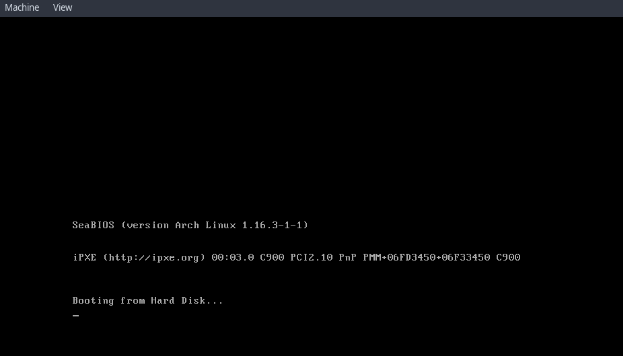
\includegraphics[scale=0.5]{boot1}

\section{Pisanje besedila v TTY načinu}
V digitalnih računalnikih je prekinitev (``interrupt'') zahteva, da procesor prekine trenutno izvajanje kode, da se nek dogodek lahko pravočasno obdela. Če je zahteva sprejeta, procesor prekine svoje trenutne dejavnosti, shrani svoje stanje in izvede funkcijo, imenovano prekinjevalnik oz. prekinjevalno servisno rutino, da izvede dogodek. Ta prekinitev je pogosto začasna, tako da lahko programska oprema nadaljuje z običajnimi dejavnostmi, ko se obdelava prekinitve konča, čeprav lahko prekinitev namesto tega pomeni usodno napako.

Implementacije BIOS-a zagotavljajo določene prekinitve, ki jih lahko operacijski sistemi in aplikacijski programi sprožijo za uporabo vdelane programske opreme v računalnikih, med njimi je tudi prekinitev za pisanje na ekran.

Naredimo operacijski sistem nekoliko bolj zanimiv s tem, da po zagonu izpiše pozdrav svetu.

V programu za oblikovanje besedila spet odprimo datoteko »hello.asm« in na začetku dodajmo naslednje vrstice:
\begin{minted}{nasm}
    mov ah, 0x0e ; v register "ah" zapiše število 0x0e
    mov al, 'P'  ; v register "al" zapiše ascii 'P'
    int 0x10     ; zažene prekinitev 0x10
\end{minted}
Ukaz v prvi vrstici pomeni premik (``move''). Prvi argument je lahko ali naslov
v spominu ali pa register v katerega bi radi premaknili naslednji argument.
``Ah'' in ``al'' predstavljata isti register, le da ``ah'' predstavlja zgornji
del registra, ``al'' pa spodnji. Argument 0x0E pomeni zapisovanje znakov v načinu TTY.

V tretji vrstici pokličemo ukaz int (``interrupt''), ki zažene prekinitev.
Podamo mu argument 0x10, ki predstavlja prekinitev za dostop do video storitev.
Da mi nebi bilo treba iste stvari ponoviti za vsako črko sem si naredil
funkcijo, v ``utils.asm'' datoteki.
\begin{minted}{nasm}
    print_string:
        pusha           ; vrednost vseh registerjev porine na "stack"
        mov bx, ax      ; vrednost ax registra premakne v bx
        mov ah, 0x0e    ; v zgornji del ax registra zapiše 0x0e
    loop:      ; definicija skoka
        mov al, [bx]    ; v al zapiše [bx]
        int 0x10        ; pokliče prekinitev 0x10
        add bx, 1       ; vrednosti v bx prišteje 1
        cmp al, 0       ; primerja ali je register al enak 0
        jne loop        ; če ni, skoči nazaj do "loop" definicije
        popa            ; vrednost registerjev zapiše nazaj iz "stacka"
        ret             ; vrne iz funkcije

    SPOROCILO: db 'Pozdrav, svet!', 0
\end{minted}
V mislih moramo imeti, da BIOS naš operacijski sistem naloži v spomin na naslovu
0x7c00 in so zaradi tega vsi naslovi, ki jih v programu uporabljamo za 0x7c00
zamaknjeni. To število bi lahko vsakič prišteli naslovu, ki ga uporabljamo, a
lažja rešitev je uporaba ``org'' direktive. Ta NASM-u pove, da so vsi naslovi zamaknjeni za 0x7c00.  Na začetek programa dodamo vrstico:
\begin{minted}{nasm}
    org 0x7c00
\end{minted}

\chapter{32-biten zaščiteni način}

\section{Kaj je zaščiteni način?}
Na žalost za naš operacijski sistem 16 bitov ne bo dovolj, potreben bo prehod na 32-biten zaščiteni način. Zaščiteni način je glavni način delovanja sodobnih Intelovih procesorjev (in klonov) od modela 80286 (16 bitov) naprej. Pri procesorjih 80386 in novejših 32-bitni zaščiteni način omogoča delo z več navideznimi naslovnimi prostori, od katerih ima vsak največ 4 GB naslovljivega pomnilnika, in sistemu omogoča strogo zaščito pomnilnika in strojne I/O zaščite ter omejevanje razpoložljivega nabora ukazov.

Procesor, ki ga inicializira BIOS, se začne v realnem načinu. Ko bom moj operacijski sistem prešel na zaščiteni način, se bo sprostila prava moč procesorja. Vendar bo uporaba večine prekinitev BIOS-a onemogočena, saj te delujejo le v realnem načinu.

\section{Prehod v 32-bitni zaščiteni način}
Ker je program začel postajati nekoliko večji sem ga razdelil v več datotek.
Začetna točka bo v datoteki ``boot\_sector.asm'', print\_string funkcijo pa sem umaknil v drugo datoteko.

Glavna oz. začetna datoteka se bo začela z ``org'' direktivo, kakor omenjeno
prej. Nato bomo pripravili računalniški sklad. Skladovni pomnilnik je mehanizem
za uporabo pomnilnika, ki omogoča, da se sistemski pomnilnik uporablja kot
začasna shramba podatkov, ki deluje po principu prvi-noter-zadnji ven. Eden od
bistvenih elementov delovanja pomnilnika sklada je register, imenovan kazalec
sklada (sp). Najprej nastavimo register bp na 0x9000, in nato register sp na
vrednost bp. Začetek sem označil z oznako ``start''.

Nato sem naredil datoteko ``protected\_mode.asm'', ki vsebuje kodo potrebno za
prehod v zaščiteni način. Prvo vsebuje funkcijo ``switch\_to\_pm'', ki izklopi
vse prekinitve, ki, kot smo omenili prej, ne bodo več uporabne. To naredi z
``cli'' ukazom.

\subsection*{GDT}
Globalna opisna tabela (GDT) je binarna podatkovna struktura, značilna za arhitekture IA-32 in x86-64. Vsebuje vnose, ki procesorju sporočajo podatke o pomnilniških segmentih. Podobna je tabela opisnikov prekinitev, ki vsebuje opisnike opravil in prekinitev.
%TODO: malo več o temu + lgdt ukaz


\begin{minted}{nasm}
; Globalna tabela deskriptorjev

; Oznaka za začetek GDT
GDT_start:  ; obvezni ničelni deskriptor
    dd 0x0  ; db definira štiri bajte
    dd 0x0

; Deskriptor kodnega segmenta
GDT_code:
    ; začetek=0x0, meja=0xfffff,
    ; 1. zastavice: prisotnost -> 1; privilegij -> 00; tip deskriptorja -> 1  (1001b)
    ; zastavice vrst: koda -> 1; skladnost -> 0; berljivost -> 1; dostopnost -> 0  (1010b)
    ; 2. zastavice: granularnost -> 1; privzeto 32-bitov -> 1; 64-bitna segmentacija -> 0; AVL -> 0  (1100b)
    dw 0xffff
    dw 0x0
    db 0x0
    db 10011010b ; 1. zastavice + zastavice vrst
    db 11001111b ; 2. zastavice + limita (biti 16-19)
    db 0x0

; Deskriptor podatkovnega segmenta
GDT_data:
    ; Enako kot pri kodnem segmentu, razen zastavic vrst:
    ; zastavice vrst: koda -> 0; razširi navzdol -> 0; zapisljivost -> 1; dostopnost -> 0  (0010b)
    dw 0xffff
    dw 0x0
    db 0x0
    db 10010010b ; 1. zastavice + zastavice vrst
    db 11001111b ; 2. zastavice + limita (biti 16-19)
    db 0x0

; Oznaka za konec GDT
GDT_end:

; Opisnik GDT (globalne tabele deskriptorjev)
GDT_descriptor:
    dw GDT_end - GDT_start - 1     ; Velikost GDT
    dd GDT_start                   ; Začetni naslov GDT

; Uporabne konstante
CODE_SEG equ GDT_code - GDT_start ; zamik kodnega segmenta
DATA_SEG equ GDT_data - GDT_start ; zamik podatkovnega segmenta
\end{minted}

Da preklopimo bo potrebno preklopiti prvi bit na posebnem kontrolnem registru
imenovanem cr0. Tega ne moremo storiti direktno, zato ga najprej naložimo v
register eax, tam naredimo spremembo in vrednost zapišemo nazaj v cr0. Nato
skočimo do funkcije ``init\_pm'', kjer nastavimo vse segmentne registre in
ponovno nastavimo stack.

\begin{minted}{nasm}
[bits 16]
switch_to_pm:
    cli                     ; izklopimo prekinitve
    lgdt [GDT_descriptor]   ; naložimo globalno tabelo deskriptorjev

    mov eax, cr0            ; vrednost kontrolnega registerja "cr0" zapišemo v eax
    or eax, 0x1             ; zadnji bit spremenimo na 1
    mov cr0, eax            ; vrednost zapišemo nazaj

    jmp CODE_SEG:init_pm    ; skok do naslednje funkcije

[bits 32]
init_pm:
    mov ax, DATA_SEG ; vse segmentne registerje
    mov ds, ax       ; nastavimo na isto vrednost,
    mov ss, ax       ; saj jih v 32 bitnem načinu ne
    mov es, ax       ; bomo uporabljali
    mov fs, ax
    mov gs, ax

    mov ebp, 0x90000 ; nastavimo stack
    mov esp, ebp

    call BEGIN_PM
\end{minted}

V glavni datoteki definiram še ``BEGIN\_PM'' funkcijo.
\begin{minted}{nasm}
[bits 32]
BEGIN_PM:
    call KERNEL_OFFSET ; pokličemo v jedro

    jmp $              ; ko jedro preneha z izvajanjem, počakamo
\end{minted}


\chapter{Jedro}

\section{Teorija}
Obstajajo različne zasnove arhitekture jedra. Monolitna jedra se v celoti
izvajajo v enem naslovnem prostoru, pri čemer se procesor izvaja v nadzornem
načinu, predvsem zaradi hitrosti. Mikro-jedra izvajajo večino svojih storitev,
vendar ne vseh, v uporabniškem prostoru, podobno kot uporabniški procesi,
predvsem zaradi odpornosti in modularnosti. MINIX 3 je pomemben primer zasnove
mikrojadra. Jedro Linuxa je hkrati monolitno in modularno, saj lahko med
izvajanjem vstavlja in odstranjuje module jedra, ki jih je mogoče naložiti.
Jedo, ki ga bom zasnoval za svoj operacijski sistem bo zelo preprosto, služil bo
kot dokaz koncepta.

Delo bi lahko nadaljeval v assemblerju, a pomanjkljivost assemblerja je, da je
tesno povezan z določeno arhitekturo procesorja, zato bi bilo težje prenesti
naš operacijski sistem na drugo arhitekturo procesorjev (npr. ARM, RISC, PowerPC).
Na srečo obstajajo alternative. To so višji jeziki (npr. FORTRAN, C, Pascal,
BASIC itd.), ki so bolj intuitivni. Za ta projekt sem se odločil za C. 

\section{Osnova}
Naredil sem novo datoteko, sedaj s končnjico ``.c". V njej sem začel pisanje jedra s tem, da sem
napisal preprosto funkcijo ``kernel, " ki izpiše `X' na ekranu.
    \begin{minted}{c}
    void kernel() {
        char *videoMemory = (char *)0xb8000;

        *videoMemory = 'X';
    }
    \end{minted}

\section{Kompilacija}
To C datoteko je treba prevesti v računalniku razumljivo kodo. Za to bom uporabil progam gcc.
Da bo prevajanje potekalo lažje sem si naredil Makefile, to je datoteka, v katero zapišem načrt
kako bo potekalo prevajanje in povezovanje mojega programa.
\inputminted{make}{../Makefile}

\chapter{Sklep}
Repozitorij: \url{https://github.com/Golobii/matura-os}

% Bibliografija
\addcontentsline{toc}{chapter}{Literatura}
\printbibliography

\end{document}
